\chapter{Theory}

\cite{goodman2000,goodman2007,agarwal2013,classen2017,cowley1995,born1980,trigg2005,attwood1999,griffiths2005,agarwal2013,classen2017,loudon2000,mandel1995,hanburry1956,galuber2006,baym1997,zernike1938,rosen96,yabashi2002,singer2013,santra2009,krause1979,trost2020,inoue2019,sorum1987,lajunen04,mpccd,tono2013}

random process
ergodic: time average equals expectation value
stationary: shifting all time instants by $\tau$ does not change the statistical description of the random process 

\section{Coherence}
Spherical waves as  solutions to wave equation
\begin{equation}
	E(\vec{r},t)=E_0(k,t) \frac{e^{i\vec{r}\vec{k}-iwt}}{R}
	\end{equation}

Superposition principle of the waves with the real amplitudes $A_{1,2}$ and phases $\phi{1,2}$
\begin{equation}
E(\vec{r},t)=E_1(\vec{r},t)+E_2\vec{r},t)=A_1*e^{i\phi_1} * e^{i\vec{r}\vec{k_1}-iw_1t} + A_1*e^{i\phi_1} * e^{i\vec{r}\vec{k_2}-iw_2t} 
\end{equation} 

measured Intensity with measurement time $T\gg1/w$
\begin{equation}
	I(\vec{r},t)\propto \int_0^T \left|E(\vec{r},t)\right|^2 \diff t
\end{equation}
Consider monochromatic light

Superposition of two monochromatic, stationary waves with a fixed phase difference $\Delta \phi$ gives rise to interference fringes
\begin{equation}
	\left<I(\vec{r},t)\right>=I_1+I_2+2\sqrt{I_1I_2}\cos\left((\vec{k_1}-\vec{k_2})\vec{r}+\Delta \phi\right)
\end{equation}

Defining the contrast of the fringes as the visibility $V$,
\begin{equation}
	V=\frac{I_{max}-I_{min}}{I_{max}+I_{min}}
\end{equation} 

Gives $V=\frac{2\sqrt{I*I}}{I+I}I=1$.

To consider non monochromatic waves we define self coherence function $\Gamma$ as 
\begin{equation}
\Gamma(\tau)=\left< E(t)E(t+\tau)\right>
\end{equation}
and its normalized version, the complex degree of coherence $\gamma$ as
\begin{equation}
\gamma(\tau)=\frac{\Gamma(\tau)}{\Gamma(0)} =  \frac{\Gamma(\tau)}{<I>}
\end{equation}



The coherence time is defined as 
\begin{equation}
\tau_c = \int_{-\infty}^{\infty} \left| g_1(\tau)\right|^2 \diff \tau 
\end{equation}





\paragraph{First order coherence $g_1$}
Generalization of$\gamma$  for to different fields  $E_1^*(\vec{r}_1,t_1)$ and $E_2(\vec{r}_2,t_2)$ is $g_1$
\begin{equation}
	g^{(1)}(\vec{r}_1,t_1;\vec{r}_2,t_2= \frac
	{\left< E_1^*(\vec{r}_1,t_1)E_2(\vec{r}_2,t_2) \right>}
	{\left[ \left<\left | E(\vec{r}_1,t_1)\right |^2 \right> \left< \left |E(\vec{r}_2,t_2)\right |^2 \right>\right]^{1/2}}	
\end{equation}






In an interferometer, light coming from a source and a time delayed copy are superposed.



For an exponentially decaying electric field $E(t)=\Theta(t)e^{-t/\tau}$, the spectrum is Lorentian with an angular frequency FWHM of $\frac{2}{\tau}$ as 
\begin{equation*}
\left|\int_{0}^{\infty}  e^{-t/\tau} e^{-iwt} \dif t \right|^2 \propto  \frac{1}{1/\tau^2+w^2} .
\end{equation*}
Therefore, an Lorentian spectrum with a FWHM of $\Delta E$ corresponds to an lifetime of $\frac{2\hbar}{\Delta E}$.

Wiener Khinchin to get g1

On the other hand, for a Lorentzian light source, $<g_1(\tau)>=e^{-|\tau/| \tau_c}$, defining the coherence time $\tau_c$ as the time, after which $g^1$ has decreased to $e^{-1} g^1(0)$.

 \begin{figure}
	\centering
	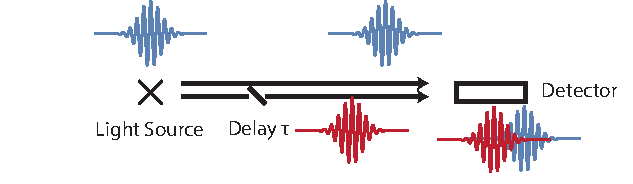
\includegraphics[width=0.8\linewidth]{images/michelson.pdf}
	\caption[Schematic of interferometer]{Schematic of interferometer: Light of (a gaussian) light source with finite coherence time is split and interference with a delayed copy is observed. The time averaged intensity measured by an detector changes with the delay time. }
	\label{fig:michelson}
\end{figure}

\begin{equation}
V=\left|g_1\right|
\end{equation}

Int
-along Glauber/Statistical Optics Goodman



Intensity in double slit leads to normalized degree of coherence $g_1$
Visiblity is modulus of $g_1$.

In a double slit setup (\fref{fig:doubleslit}), $E(r,t)=c_1 E_1(t)+c_2E2(t)$ with complex $c_2$ and $c_2$, $\left|c_1\right|\approx\left|c_2\right|$ describing the propagation to the screen. 

\begin{figure}
	\centering
	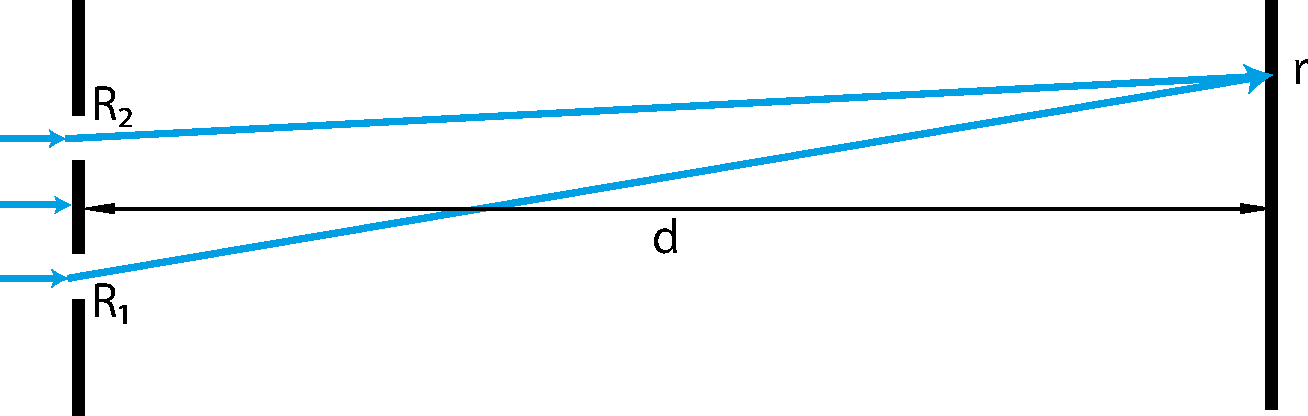
\includegraphics[width=0.8\linewidth]{images/doubleslit.pdf}
	\caption[Schematic of double slit]{Schematic of double slit: Monochromatic light goes through slits located at $R_1$ and $R_2$. The intensity at a position $r$ on the scree (in distance $d$) is the superposition of both paths.  If the slits are within the lateral coherence area of the source, the visibility of the interference pattern depends on the path length difference in comparison to the coherence time $\tau$.}
	\label{fig:doubleslit}
\end{figure}


\paragraph{Second order coherence $g_2(t_1,t_2)$}
The definition of $g_1$ can be extended to the second order by
\begin{equation*}
	g^{(2)}(\vec{r}_1,t_1;\vec{r}_2,t_2= 
	\frac{\left< E^*(\vec{r}_1,t_1)E^*(\vec{r}_2,t_2)E(\vec{r}_1,t_1)E(\vec{r}_2,t_2) \right>}{\left<\left | E(\vec{r}_1,t_1)\right |^2 \right> \left< \left |E(\vec{r}_2,t_2)\right |^2 \right>}	
\end{equation*}
For classical fields normalized correlations of intensities:
\begin{equation}
	g^{(2)}(\vec{r}_1,t_1;\vec{r}_2,t_2)= 
		\frac{\left< I(\vec{r}_1,t_1)I(\vec{r}_2,t_2 \right>}{\left<I(\vec{r}_1,t_1)\right>\left<I(\vec{r}_1,t_1)\right>}	
\end{equation}

\paragraph{Van Cittert Zernicke}

%-Hanbury Brown and Twist
\section{Hanburry Brown Twiss}
Hanburry Brown and Twiss 


\paragraph{Siegert Relation}
For thermal light, 
\begin{equation}
	g_2(\vec{r_1},\vec{r_2}) = 1+ |g_1(\vec{r_1},\vec{r_2}) |^2 ,
\end{equation}
which is called the Siegert Relation.
For $N$ Single-Photon-Emitters, a similiar form holds \cite{classen2017}:
\begin{equation}
	g_2(\vec{r_1},\vec{r_2}) = 1+ |g_1(\vec{r_1},\vec{r_2}) |^2 - \frac{2}{N} ,
\end{equation}
$g_1$ encodes structural information, as 
\begin{equation}
g_1(\vec{k_1},\vec{k_2}) \propto \mathscr{F}S(\vec{r}) = S(\vec{q})
\end{equation}
is proportional to the Fourier transform of the arangment of emitters with $q=\vec{k_1}-\vec{k_2}$ (see \fref{fig:scatteringvectors}).
 \begin{figure}
	\centering
	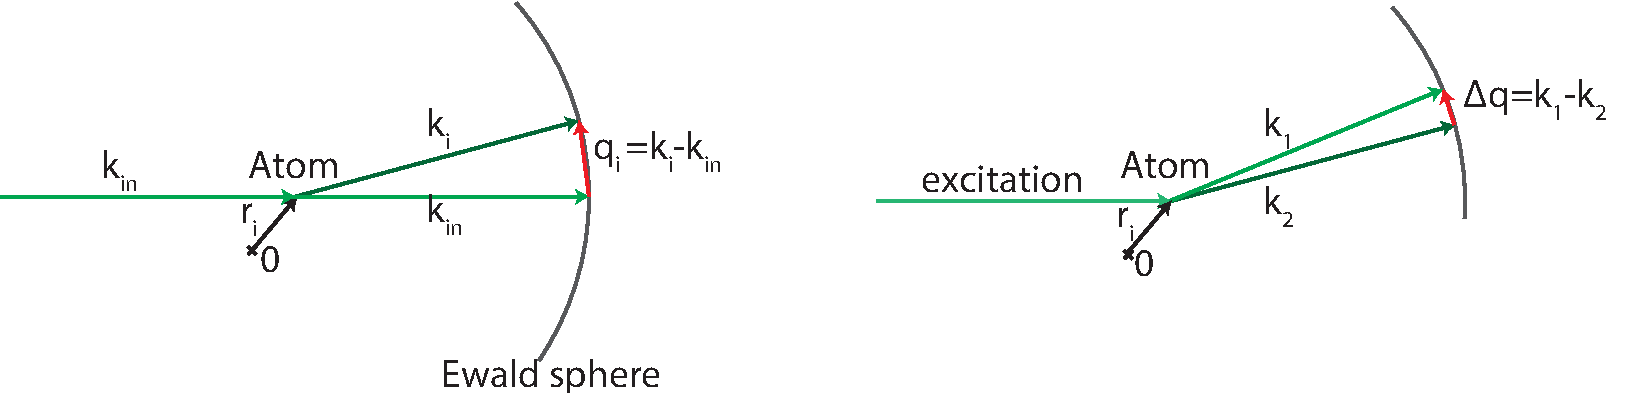
\includegraphics[width=0.9\linewidth]{images/scatteringvectors.pdf}
	\caption[Scattering Vectors]{Scattering vector $q$ in CDI (left) and IDI (right). In CDI, $q$ is the momentum transfer between incoming and outgoing wave. In IDI, there is no momentum transfer from the incoming to the outgoing wave. Instead, intensity correlations of different $k_1$, $k_2$ give a momentum transfer $\delta q$ according to the Siegert relation.}
	\label{fig:scatteringvectors}
	
\end{figure}

%-Single Photon Emitters/2nd Quant description
%(siehe Referenzen in Schaller/resonance fluorescence)
%-Fluorescence g2
%$2 Level with finite Lifetime -> Spectrum of fluorescence
\section{X-Ray Fluorescence}

\section{Intensity Correlations using X-Ray Fluorescence}
\section{Signal to Noise Considerations}
The speckle contrast is governed by the number of independent modes overlaid in the measurement.
If the measurement, happens over a finite amount of time there will, the number of temporal degrees of freedom is
\begin{equation}
M_t=\frac{\left(\int_{-\infty}^{\infty} P(t)\diff t\right)^2}{\int_{-\infty}^{\infty} K(t) \left|\mu(t)\right|^2\diff t}
\end{equation}
with $P(t)$ the integration window weighting function and $K(t)$ its autocorrelation. If the integration windows is set by the integration time $T$ of the detector, $P(t)$ is a rectangular function with the width $T$ and
\begin{equation}
M_t,rect = \frac{T}{2} \left[\int_{0}^{T} \left( 1-\frac{t}{T}\right) \left|\mu(t)\right|^2 \diff t \right]^{-1} .
\end{equation}
If instead $P(t)$ is the Gaussian excitation pulse with FWHM of $\tau$ and unit area,
\begin{align}
P(t)&=\frac{2\sqrt{\ln 2}}{\sqrt{\pi} \tau} e^{-\left(2\sqrt{\ln 2}\frac{t}{\tau}\right)^2}\\
K(t)&= \sqrt{\frac{2{\ln 2}}{\pi}}\frac{1}{ \tau} e^{-\left(\sqrt{2\ln 2}\frac{t}{\tau}\right)^2}
\end{align}
the number of degrees of freedom is
\begin{align}
M_t,gauss&=\left[\int_{-\infty}^{\infty} K(t) \left|\mu(t)\right|^2\diff t\right]^{-1}.
\end{align}
For a Lorentzian spectrum (see \fref{eq:docdecay}), this evaluates to
\begin{equation}
	Inhalt...
\end{equation} 

The experimentally indistinguishable fluorescence energies $K_\alpha,1$ and $K_\alpha,2$ (as well as  $K_\beta$ if no filter is used for suppression) give additional independent modes $M_E$

As the used X-ray detectors are polarization insensitive and X-ray fluorescence is unpolarized, there are 2 independent polarization modes giving $M_P = 2$  


Path differences longer than the coherence length give additional modes, therefore the speckle visibility will be reduced large samples:

If the speckle pattern is not spatially resolved by the detector because its resolution is to low compared to the change in intensity, undersampling will occur, the meassured signal will be spatially averaged giving independent sampling modes $M_S$





As good approximation, the total number of modes can be considered the product of those modes numbers (in reality, the mode numbers are not completely independent, see \fref{chap:simulation})
%- SNR
%will use Peak/stdev bg definition
Which factors influence SNR
-lifetime/pulsewidth
-polarisation
-sampling conditions / undersampling
-sample thickness / coherence length
-N images
-N photons
\label{chap:theory}




\section{Kossel Lines}
X-Ray radiation originating from within a single crystal gets Bragg reflected at the lattice planes, causing Intensity variation in $90^o-\theta$ around the direction $k_{hkl}$, forming the \textit{Kossel Cones}. On the spherical detector centered at at the crystal, the points with influenced intensity would lie on circles with radii determined by ...

The visibility of the Kossel lines is governed by the same extinction rules as for the Bragg reflexes for, the structure factor $F_{hkl}$ has to be non-zero. For a zinc blende structure (such as GaAs) with atomic scattering factors $f_a$ and $f_b$, the structure factor is
\begin{align}
F_{hkl} = \begin{cases}
0, & \text{if $h$, $k$, $l$ mixed parity}.\\
4(f_a+f_b), & \text{if same parity and $h+k+l = 4 N$} \\
4(f_a\pm i f_b), & \text{if same parity and $h+k+l = 2 N+1$} \\
4(f_a-f_b), & \text{if same parity and $h+k+l = 4 N+2$} \\
\end{cases}
\end{align}

The structure of the intensity variations (both intense and less intense depends on the which case...
If the fine structure cannot be resolved

The Kossel lines allow to orient the detector with regards to the lattice planes. This can either be done by reprojecting the planar detector onto a sphere by an inverse gnomonic projection and determining circle center and radius, eg. by an Hugh-Transform, or by a fitting conic sections to the lines on the planar detector. As the observable curvature of the Kossel lines on the detector in an IDI setup is small and therefore the circles are difficult to determine, the second method will be used. 

As each point identifyed as beloning to a Kossel line has to be part of a conic section of the same plane with each cone originating from the same point, each point $r$ on a line has to fullfill



\begin{equation}
\frac{\vec{r} \cdot \vec{q}}{\left|\vec{r}\right| \left| \vec{q}\right|} = \frac{\lambda}{2d}
\end{equation}
 for a reciprocal lattice vector $q$ which is an element of the allow reflections $Q$. So finding the dector orientation can be seen as finding a rotation Matrix $R$ as
\begin{equation}
\arg\!\min_{R} \sum_{r} \min_{q\in Q} \frac{2 d * \vec{r} \cdot \vec{Rq}}{\left|\vec{r}\right| \left| \vec{q}\right|} -\lambda
\end{equation}
\begin{figure}
	\centering
	\begin{subfigure}[b]{0.25\textwidth}
	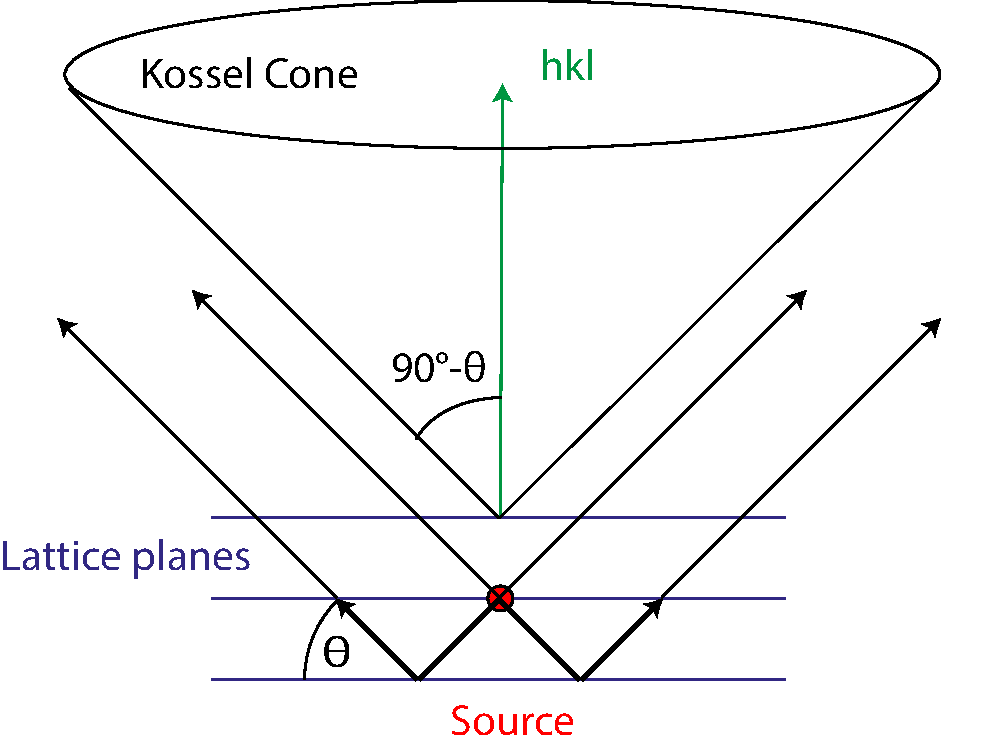
\includegraphics[width=\linewidth]{images/kossel0.pdf}
	\end{subfigure}
	\begin{subfigure}[b]{0.25\textwidth}
	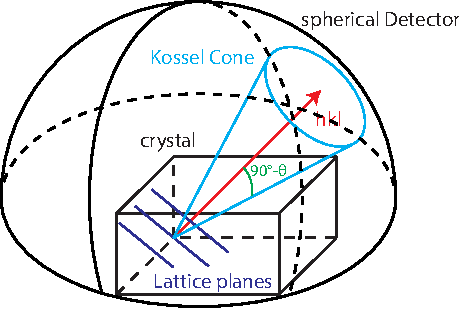
\includegraphics[width=\linewidth]{images/kossel.pdf}
	\end{subfigure}
	\begin{subfigure}[b]{0.35\textwidth}
	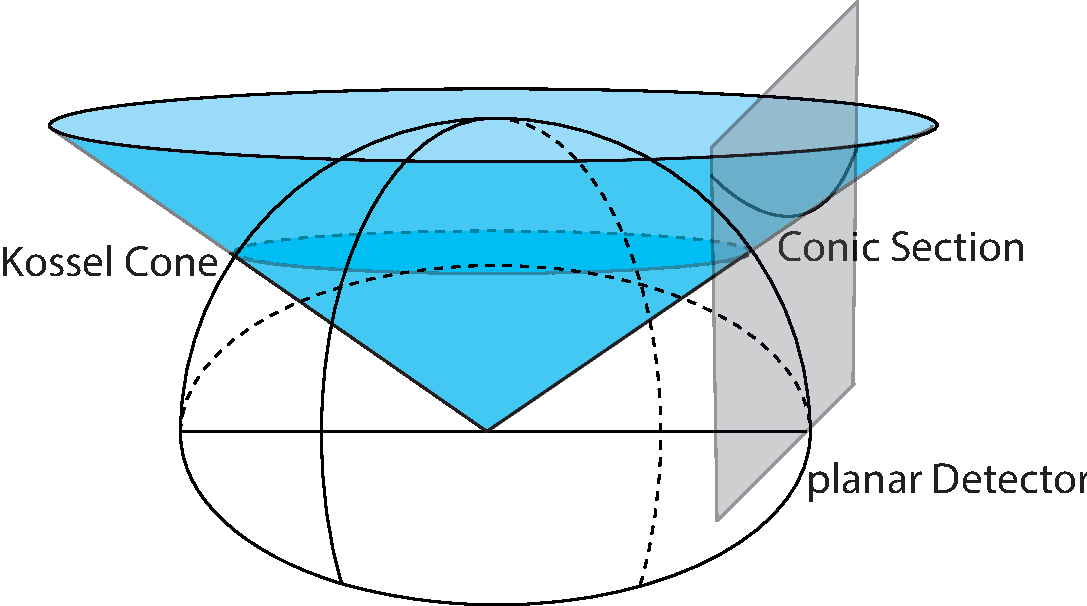
\includegraphics[width=\linewidth]{images/kossel2.pdf}
	\end{subfigure}
	\caption[Geometry of Kossel Lines]{Geometry of Kossel Lines: Radiation from within a light source within a single crystal gets scattered at the lattice planes, causing a change in intensity along a cone of opening angle $90^o-\theta_{hkl}$ and vertex hkl (left). On a spherical detector centered around the sample, those intensity changes would be visible as circular Kossel lines (center). On a planar detector, the intersections of the Kossel cones are visible as conic sections (right)}
	\label{fig:doubleslit}
\end{figure}